\chapter{Outer Product}

The outer product is an expansion operation. 
Two vectors give a matrix containing the vectors' dimensions; 
the dimensions where the two vectors were having one dimension and transform it into two-dimension.


Let $x$ and $y$ be the vectors of length $n$ and $m$ respectively.

\vspace*{0.5 cm}
$x = 
\begin{bmatrix}
    x_0 \\    
    x_1 \\    
    \vdots \\
    x_n \\    
\end{bmatrix}
,\ y = 
\begin{bmatrix}
    y_0 \\    
    y_1 \\    
    \vdots \\
    y_n \\    
\end{bmatrix}
$

\begin{equation}
    A = x \otimes y^T
    \label{eq:org_outer_prod}
\end{equation}
Or
\begin{equation}
    A = x \otimes y^T + A
    \label{eq:outer_prod}
\end{equation}

\[
\begin{bmatrix}
    x_0 \\    
    x_1 \\    
    \vdots \\
    x_n \\    
\end{bmatrix}
\otimes 
\begin{bmatrix}
    y_0 &   y_1 &    \dots &   y_n
\end{bmatrix}
=
\begin{bmatrix}
    x_0 \times y_0  & x_0 \times y_1    & \dots     & x_0 \times y_n \\
    x_1 \times y_0  & x_1 \times y_1    & \dots     & x_1 \times y_n \\
    \vdots          & \vdots            & \ddots    & \vdots \\
    x_n \times y_0  & x_n \times y_1    & \dots     & x_n \times y_n \\
\end{bmatrix}
\]

Where $A$ is the resultant matrix of dimensions $n$ and $m$.

The routine \textbf{?ger} implements the equation \ref{eq:outer_prod}, 
so we are doing the same. Once we implement the operation for one layout, 
another layout found using the exact implementation by rearranging 
the inputs. For example, if the implementation uses the column-major 
layout, then the row-major can be obtained by taking the matrix's 
transpose or exchanging the vectors

Taking the transpose on the both side in equation \ref{eq:outer_prod}.
\[A^T = (x \otimes y^T + A)^T\]

Transpose on the matrix addition is distributive, so we get
\[A^T = (x \otimes y^T)^T + A^T\]

We can transpose inside the outer product, but the vectors exchange 
their position and transpose self-cancellation operation.

\begin{equation}
    A^T = y \otimes x^T + A^T
    \label{eq:outer_prod_trans}
\end{equation}

If $A$ is a column-major then $A^T$ is must be row-major and vice-versa.

\section{Algorithm}

\begin{figure}[htb]
    \centering
    \subfloat[\centering Block Diagram]{{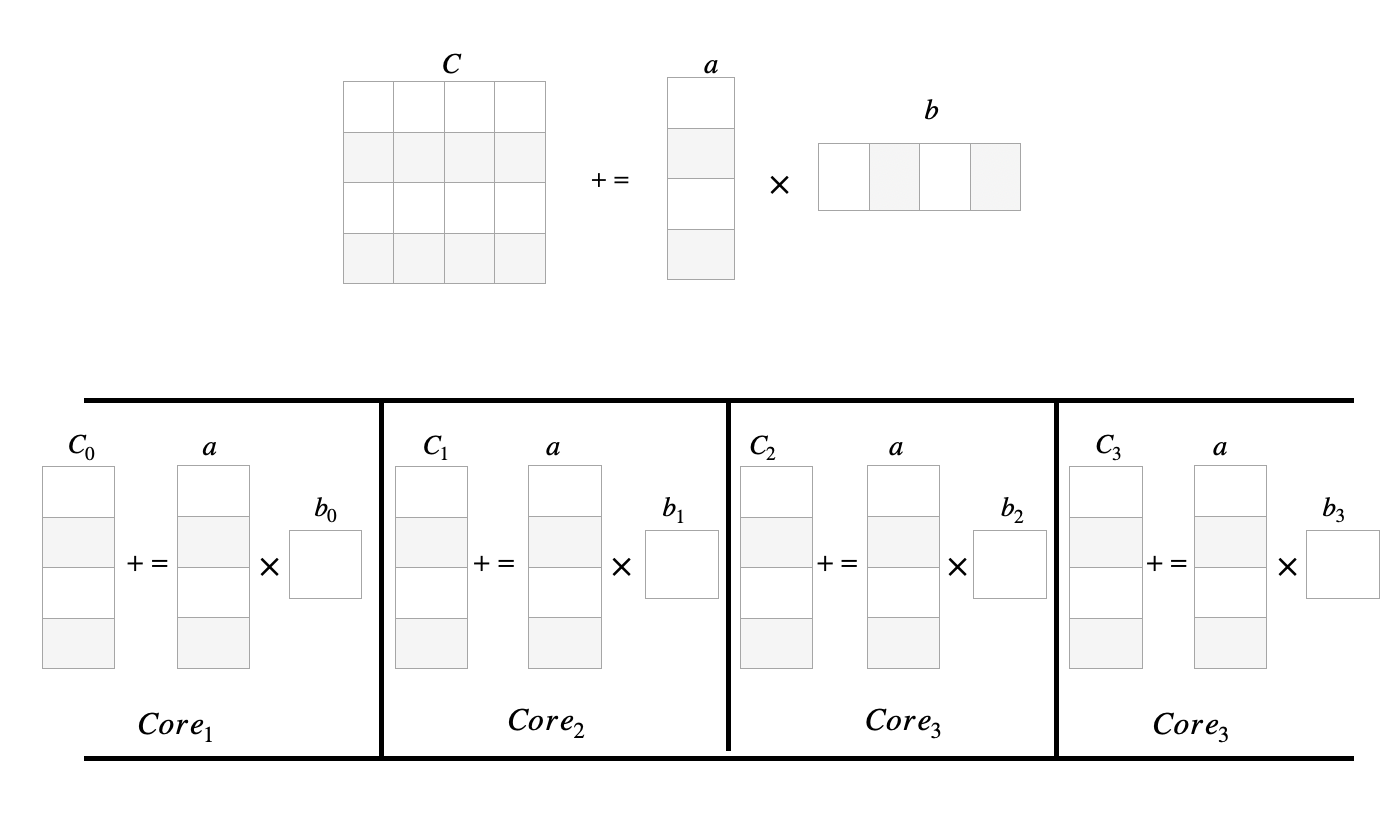
\includegraphics[width=10cm]{../assets/outer_product/Algo_visual.png} }}%
\end{figure}

\begin{algorithm}[H]
    \SetAlgoLined
    \SetKwFunction{SIMDFn}{outer\_simd\_loop}
    \SetKwProg{Fn}{Function}{:}{end}

    \tcp{$c$ is the pointer to the output matrix}
    \tcp{$a$ is the pointer to the first vector}
    \tcp{$b$ is the pointer to the second vector}
    \tcp{$n$ is the length of the vectors}
    \Fn{\SIMDFn($c$, $a$, $b$, $n$)}{
        \assignln{cst}{b[0]}

        \openmp{simd}
        \For{\assign{i}{0} \KwTo $n$ \KwBy 1}{
            \assignln{c[i]}{c[i] + a[i] \times cst}
        }
        \KwRet{$sum$}
    }
    \caption{Outer Product SIMD Function}
\end{algorithm}

\begin{algorithm}[H]
    \SetAlgoLined
    \KwIn{$c, wc, a, na, b, nb, max\_threads$}
    \tcp{$a$ and $b$ are vectors}
    \tcp{$c$ is the pointer to the output matrix}
    \tcp{$na$ is the size of the vector $a$}
    \tcp{$nb$ is the size of the vector $b$}
    \tcp{$wc$ is the leading dimension of the matrix $c$}
    \tcp{$max\_threads$ is the user provided thread count}
     \Begin{
        \assignln{MinSize}{256}
        \assignln{number\_el\_L_2}{\lfloor \frac{S_{L_2}}{S_{data}} \rfloor}
        \assignln{upper\_limit}{\lfloor \frac{number\_el\_L_2 - na}{na} \rfloor}
        \assignln{num\_threads}{max(1,min(upper\_limit,max\_threads))}
        $omp\_set\_num\_threads(num\_threads)$

        \openmp{parallel for if($nb$ $>$ $MinSize$)}
        \For{$i\gets 0$ \KwTo $ nb $ \KwBy $1$}{
            $aj \gets a$ \\
            $bj \gets b + i$ \\
            $cj \gets b + i \times wc $ \\
            $outer\_simd\_loop$($cj$, $aj$, $bj$, $na$);\\
        }
     }
    \caption{Vector-Vector Outer Product}
\end{algorithm}